\documentclass[tikz,border=6pt]{standalone}
\usepackage{amsmath,amssymb}
\usetikzlibrary{arrows.meta,positioning}
\definecolor{accentA}{HTML}{2E7D5B}
\begin{document}
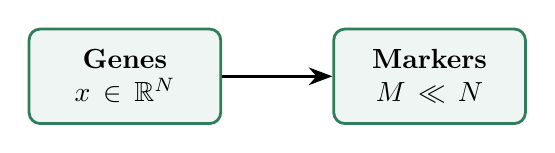
\begin{tikzpicture}
\node[rounded corners,draw=accentA,line width=1pt,fill=accentA!8,text width=22mm,align=center,minimum height=12mm] (a){\textbf{Genes}\\ $x\in\mathbb{R}^N$};
\node[rounded corners,draw=accentA,line width=1pt,fill=accentA!8,right=14mm of a,text width=22mm,align=center,minimum height=12mm] (b){\textbf{Markers}\\ $M\ll N$};
\draw[-{Stealth[length=3mm]},line width=1pt] (a)--(b);
\end{tikzpicture}
\end{document}
